% mnras_template.tex 
%
% LaTeX template for creating an MNRAS paper
%
% v3.0 released 14 May 2015
% (version numbers match those of mnras.cls)
%
% Copyright (C) Royal Astronomical Society 2015
% Authors:
% Keith T. Smith (Royal Astronomical Society)

% Change log
%
% v3.0 May 2015
%    Renamed to match the new package name
%    Version number matches mnras.cls
%    A few minor tweaks to wording
% v1.0 September 2013
%    Beta testing only - never publicly released
%    First version: a simple (ish) template for creating an MNRAS paper

%%%%%%%%%%%%%%%%%%%%%%%%%%%%%%%%%%%%%%%%%%%%%%%%%%%%%%%%%%%%%%%%%%%%%%%%%%%%%%%%
% Basic setup. Most papers should leave these options alone.
\documentclass[fleqn,usenatbib]{mnras}

% MNRAS is set in Times font. If you don't have this installed (most LaTeX
% installations will be fine) or prefer the old Computer Modern fonts, comment
% out the following line
\usepackage{newtxtext,newtxmath}
% Depending on your LaTeX fonts installation, you might get better results with one of these:
%\usepackage{mathptmx}
%\usepackage{txfonts}

% Use vector fonts, so it zooms properly in on-screen viewing software
% Don't change these lines unless you know what you are doing
\usepackage[T1]{fontenc}

% Allow "Thomas van Noord" and "Simon de Laguarde" and alike to be sorted by "N" and "L" etc. in the bibliography.
% Write the name in the bibliography as "\VAN{Noord}{Van}{van} Noord, Thomas"
\DeclareRobustCommand{\VAN}[3]{#2}
\let\VANthebibliography\thebibliography
\def\thebibliography{\DeclareRobustCommand{\VAN}[3]{##3}\VANthebibliography}


%%%%% AUTHORS - PLACE YOUR OWN PACKAGES HERE %%%%%

% Only include extra packages if you really need them. Common packages are:
\usepackage{graphicx}	% Including figure files
\usepackage{amsmath}	% Advanced maths commands
% \usepackage{amssymb}	% Extra maths symbols
\usepackage{multirow}
\usepackage{svg}
\usepackage{tabularx}
%%%%%%%%%%%%%%%%%%%%%%%%%%%%%%%%%%%%%%%%%%%%%%%%%%%%%%%%%%%%%%%%%%%%%%%%%%%%%%%%

%%%%% AUTHORS - PLACE YOUR OWN COMMANDS HERE %%%%%

% Please keep new commands to a minimum, and use \newcommand not \def to avoid
% overwriting existing commands. Example:
%\newcommand{\pcm}{\,cm$^{-2}$}	% per cm-squared
\newcommand{\msun}{\mathcal{M}_{\sun}}
\newcommand{\orcid}[1]{\href{https://orcid.org/#1}{\includesvg[width=10pt]{orcid}}}

\newcommand{\dummyfig}[1]{
  \centering
  \fbox{
    \begin{minipage}[c][0.25\textheight][c]{\columnwidth}
      \centering{#1}
    \end{minipage}
  }
}

\setlist[enumerate]{wide=0pt, widest=99, leftmargin=\parindent, labelsep=*}

%%%%%%%%%%%%%%%%%%%%%%%%%%%%%%%%%%%%%%%%%%%%%%%%%%%%%%%%%%%%%%%%%%%%%%%%%%%%%%%%

%%%%%%%%%%%%%%%%%%%%%%%%%%%%%%%%%% TITLE PAGE %%%%%%%%%%%%%%%%%%%%%%%%%%%%%%%%%%

% Title of the paper, and the short title which is used in the headers.
% Keep the title short and informative.
\title[Galactic SFH from Gaia GCNS WDLF]{A new method to retrieve the star formation history from white dwarf luminosity functions -- an application to the $Gaia$ catalogue of nearby stars}

% The list of authors, and the short list which is used in the headers.
% If you need two or more lines of authors, add an extra line using \newauthor
%\author[M. C. Lam et al.]{
%M. C. Lam$^{1\,\orcid{0000-0002-9347-2298}}$\thanks{Contact e-mail: \href{mailto:lam@mail.tau.ac.il}{lam@tau.ac.il}}
%\\
\author[M. C. Lam et al.]{
M. C. Lam$^{1, 2}$\thanks{Contact e-mail: \href{mailto:mlam@roe.ac.uk}{mlam@roe.ac.uk}},
and N. Rowell$^{2}$
\\
% List of institutions
$^{1}$School of Physics and Astronomy, Tel Aviv University, Tel Aviv, Israel 69978\\
$^{2}$Institute for Astronomy, University of Edinburgh, Royal Observatory, Blackford Hill, Edinburgh EH9 3HJ, UK
}

% These dates will be filled out by the publisher
\date{Accepted XXX. Received YYY; in original form ZZZ}

% Enter the current year, for the copyright statements etc.
\pubyear{2023}

% Don't change these lines
\begin{document}
\label{firstpage}
\pagerange{\pageref{firstpage}--\pageref{lastpage}}
\maketitle

%%%%%%%%%%%%%%%%%%%%%%%%%%%%%%%%%%%%%%%%%%%%%%%%%%%%%%%%%%%%%%%%%%%%%%%%%%%%%%%%

% Abstract of the paper
\begin{abstract}
With the state-of-the-art Gaia astrometry, the number of confirmed white dwarfs
has reached a few hundred thousand. We have reached the era where small features
in the white dwarf luminosity function~(WDLF) of the solar neighbourhood can be
resolved. We demonstrate how to apply Markov chain Monte Carlo sampling on a
set of pre-computed partial-WDLFs to derive the star formation history of their
progenitor stellar population. We compare the results against many well-accepted
and established works using various types of stars, including white dwarfs,
main sequence stars, sub-giants and the use of the entire stellar population
available to their data. We find convincing agreements among most of the
methods, particularly at the intermediate age of 1-8\,Gyr.

\end{abstract}

% Select between one and six entries from the list of approved keywords.
% Don't make up new ones.
\begin{keywords}
keyword1 -- keyword2 -- keyword3
\end{keywords}

%%%%%%%%%%%%%%%%%%%%%%%%%%%%%%%%%%%%%%%%%%%%%%%%%%%%%%%%%%%%%%%%%%%%%%%%%%%%%%%%

%%%%%%%%%%%%%%%%%%%%%%%%%%%%%%%%% BODY OF PAPER %%%%%%%%%%%%%%%%%%%%%%%%%%%%%%%%

\section{Introduction}
%%%%%%%%%%%%%%%%%%%%%%%%%%%%%%%%%%%%%%%%%%%%%%%%%%%%%%%%%%%%%%%%%%%%%%%%%%%%%%%%
White dwarfs~(WDs) are the final stage of stellar evolution of main
sequence~(MS) stars with zero-age MS~(ZAMS) mass less than $8\msun$. Since this
mass range encompasses the vast majority of stars in the Galaxy, these
degenerate remnants are the most common final product of stellar evolution,
thus these are a good population to study the history of star formation in the
Galaxy. In this state, there is little nuclear burning to replenish the energy
they radiate away. As a consequence, the luminosity and temperature decrease
monotonically with time. The electron degenerate nature means that a WD with a
typical mass of $0.6\mathcal{M}_{\sun}$ has a similar size to the Earth, giving
rise to their high densities, low luminosities, and large surface gravities.

%%%%%%%%%%%%%%%%%%%%%%%%%%%%%%%%%%%%%%%%%%%%%%%%%%%%%%%%%%%%%%%%%%%%%%%%%%%%%%%%
The use of the white dwarf luminosity function~(WDLF) as a cosmochronometer was
first introduced by \citet{1959ApJ...129..243S}. Given the finite age of the
Galaxy, there is a minimum temperature below which no white dwarfs can reach in
a limited cooling time. This limit translates to an abrupt downturn in the WDLF
at faint magnitudes. Evidence of such behaviour was observed by
\citet{1979ApJ...233..226L}, however, it was not clear at the time whether it
was due to incompleteness in the observations or to some defect in the
theory~(e.g.,~\citealp{1984ApJ...282..615I}). A decade later,
\citet{1987ApJ...315L..77W} gathered concrete evidence for the downturn and
estimated the age\footnote{``Age'' refers to the total time since the oldest
WD progenitor arrived at the zero-age main sequence.} of the disc to be
$9.3 \pm 2.0$\,Gyr~(see also \citealt{1988ApJ...332..891L}). While most studies
focused on the Galactic discs~\citep{1989LNP...328...15L, 1992ApJ...386..539W,
1995LNP...443...24O, 1998ApJ...497..294L, 1999MNRAS.306..736K,
2012ApJS..199...29G, 2021A&A...649A...6G}, some worked with the stellar
halo~\citep{2006AJ....131..571H, 2011MNRAS.417...93R, 2017AJ....153...10M,
2019MNRAS.482..715L, 2021MNRAS.502.1753T}.
 
%%%%%%%%%%%%%%%%%%%%%%%%%%%%%%%%%%%%%%%%%%%%%%%%%%%%%%%%%%%%%%%%%%%%%%%%%%%%%%%%
Most WDs have similar broadband colour to main sequence stars, they cannot be
identified using photometry alone. They are found from UV-excess, large
proper motion and/or parallax. Because of the strongly peaked surface gravity
distribution of WDs, photometric fitting for their intrinsic properties
is possible by assuming a surface gravity. WDs fitted in such a way are useful
statistically provided that the sample is not strongly selection biased. This
is demonstrated in various studies comparing photometric and spectroscopic
solutions to calibrate the atmosphere
model~\citep{2019ApJ...871..169G, 2019ApJ...882..106G}, as well as from the
agreeing shapes of the WDLFs from spectroscopic and photometric samples. The
Gaia satellite provides parallactic measurements for over a billion point
sources~\citep{2021A&A...649A...1G, 2021AJ....161..147B} of which $359,000$
are high confidence WD candidates~\citep[][hereafter, GF21]{2021MNRAS.508.3877G}.
The availability of parallaxes allows much more accurate fitting, particularly
important when the surface gravity is unknown for the photometric sample. This
has completely revolutionized the field of WD sciences. 

%%%%%%%%%%%%%%%%%%%%%%%%%%%%%%%%%%%%%%%%%%%%%%%%%%%%%%%%%%%%%%%%%%%%%%%%%%%%%%%%
The Early Data Release 3~(EDR3) of $Gaia$ relies on 34 months of observations, it
represents an improvement on all fronts over DR2, with parallax measurements
being now on average 20-30 per cent more accurate and proper motion measurements
twice as accurate as in the previous
DRs~\citep{2021A&A...649A...1G, 2021A&A...649A...2L}. The $Gaia$ Catalogue of
Nearby Stars~(GCNS) contains 331\,312 objects within 100\,pc of the Sun, of
which 21\,848 are white dwarfs~\citep{2021A&A...649A...6G}.

%%%%%%%%%%%%%%%%%%%%%%%%%%%%%%%%%%%%%%%%%%%%%%%%%%%%%%%%%%%%%%%%%%%%%%%%%%%%%%%%
This article is organized as follows: in Section~2, we go through the background
of WDLFs; in Section~3 we explain how WDs can be used to retrieve the SFH of a
population and introduce a new concept -- partial WDLF. We explain the fitting
procedure in Section~4 and then apply it to the $Gaia$ data in Section~5. In
Section~6 we compare the results against previous works. We conclude and discuss
potential future work in Section~7.

\section{White Dwarf Luminosity Function}
%%%%%%%%%%%%%%%%%%%%%%%%%%%%%%%%%%%%%%%%%%%%%%%%%%%%%%%%%%%%%%%%%%%%%%%%%%%%%%%%
WDLF is a common tool for deriving the age of a stellar population. A WDLF is
the number density of WD as a function of luminosity, it is an evolving
function with time. Its shape and normalisation are determined from only a few
parameters. \citet{1987ApJ...315L..77W} compared an observed WDLF derived from
the Luyten Half-Second~(LHS) catalogue with a theoretical WDLF to obtain an
estimate of the age of the Galaxy for the first time with this technique.
\citet{1990ApJ...352..605N} examined WDLFs with various SFH scenarios. They
showed that WDLF is a sensitive probe of the star formation history~(SFH) as
it shows signatures of irregularities in the SFH such as bursts and lulls.
\citet{2013MNRAS.434.1549R} took it further to address this inverse problem
mathematically and showed some success in recovering the SFH of the solar
neighbourhood when compared against SFH computed from other methods. By
decomposing the disks and halo components of the Milky Way, we can have an
independent view of the past star formation history revealed by only the
WD populations, where they are most useful in deriving the SFH of old
stellar populations~\citep{2011MNRAS.417...93R, 2017ASPC..509...25L}.

%%%%%%%%%%%%%%%%%%%%%%%%%%%%%%%%%%%%%%%%%%%%%%%%%%%%%%%%%%%%%%%%%%%%%%%%%%%%%%%%
The physical picture of getting a population of isolated WDs is
straightforward: the progenitor stars formed in their birth clusters
following a distribution of mass~($\mathcal{M}_i$) described by the initial
mass function~(IMF, $\phi$). Then, they spend their lifetime carrying out
nuclear burning~($t_{\mathrm{MS}}$), and the time they spend depends mainly
on their mass. Towards the end stage of stellar evolution, stars loses most
of the atmosphere, modelled by the initial-final mass relation~(IFMR,
$\zeta$). Once they have become WDs, all that is left is to know how long it
has been cooling~($t_{\mathrm{cool}}$) in order to reach the current
luminosity~($M_\mathrm{bol}$). Most of the computations to account for these
physical processes are coming from the interpolations of pre-computed lookup
tables. Particular care is needed to interpolate and integrate over the
grids of WD evolutionary models, because they are both susceptible to
significant rounding errors given the huge dynamic ranges the variables cover.
For example, in the case of a simple starburst of $\mathcal{O}(10^6)$\,yrs, it
requires a relative error tolerance of $10^{-10}$ in order to integrate properly
for an old population.

%%%%%%%%%%%%%%%%%%%%%%%%%%%%%%%%%%%%%%%%%%%%%%%%%%%%%%%%%%%%%%%%%%%%%%%%%%%%%%%%
When the function is \textit{properly} smoothed and weighted, and the
uncertainties accurately propagated, the parameterization using luminosity or
magnitude should give identical results agreed to within the errors coming from
the interpolation over the model grid covering a large dynamic range of values.
In this work, we parametrize the computation with the bolometric magnitude. The
integral for a WDLF when parameterised with bolometric magnitude can be written
as

\begin{equation} \label{eqn:wdlf}
    n(M_{\mathrm{bol}}) = \int_{\mathcal{M}_l}^{\mathcal{M}_u}
        \tau(M_\mathrm{bol}, \mathcal{M}_f)
        \psi(T_0, M_\mathrm{bol}, \mathcal{M}_i, \mathcal{M}_f, Z)
        \phi(\mathcal{M}_i) d\mathcal{M}_i
\end{equation}
where $n$ is the number density, $\tau$ is the inverse cooling rate, $\psi$ is
the relative star formation rate, $\phi$ is the initial mass function; and their
dependent variables: $M_\mathrm{bol}$ is the absolute bolometric
magnitude, $\mathcal{M}_f$ is the WD mass, $T_0$ is the look-back time, $\mathcal{M}_i$ is
the progenitor MS mass, $Z$ is the metallicity, $\mathcal{M}_l$ is the minimum
progenitor MS mass that could have singly evolved into a WD in the given time,
and $\mathcal{M}_u$ is the maximum progenitor MS mass.

%%%%%%%%%%%%%%%%%%%%%%%%%%%%%%%%%%%%%%%%%%%%%%%%%%%%%%%%%%%%%%%%%%%%%%%%%%%%%%%%
The inverse cooling rate
\begin{equation}
    \tau(M_\mathrm{bol}, \mathcal{M}_f) = \dfrac{dt_{\mathrm{cool}}}{dM_\mathrm{bol}} \left( M_\mathrm{bol}, \mathcal{M}_f \right)
\end{equation}
is a quantity taken from the pre-computed grid of cooling models. This rate is
also dependent on the internal structure and the chemistry of the core as well
as the atmosphere of the WDs. However, interpolation over these dependency is
not possible with the available models so their effects are not included in
this work, and is not included in the equation.

The relative star formation rate is expressed as a function of look-back time,
\begin{align}
    &\psi(T_0, M_\mathrm{bol}, \mathcal{M}_i, \mathcal{M}_f, Z) =\\
    &\qquad\psi\left[T_0 - t_{\mathrm{cool}}\left(M_\mathrm{bol}, \mathcal{M}_f\right) - t_{\mathrm{MS}}\left(\mathcal{M}_i, Z\right)\right]
\end{align}
where $\psi$ is set to zero when $T_{0}$ exceeds the total time spent on the
main sequence evolution and the WD cooling time~(i.e.\ the onset of star 
formation). The absolute normalisation is not needed when the total stellar
mass is coming from observations; the theoretical WDLF only needs to multiply
with a constant (the total number density) to account for the normalisation.

%%%%%%%%%%%%%%%%%%%%%%%%%%%%%%%%%%%%%%%%%%%%%%%%%%%%%%%%%%%%%%%%%%%%%%%%%%%%%%%%
The IFMR takes a simple form of
\begin{equation}
    \mathcal{M}_f = \zeta(\mathcal{M}_i),
\end{equation}
although there is evidence that more metal-rich stars lose more
envelope~\citep{2007ApJ...671..761K}, there is insufficient empirical data
to derive an IFMR at metallicity much lower or higher than solar abundance.

%%%%%%%%%%%%%%%%%%%%%%%%%%%%%%%%%%%%%%%%%%%%%%%%%%%%%%%%%%%%%%%%%%%%%%%%%%%%%%%%
All the calculations in this work adopt the following models: the IMF is that of
\citet{2003PASP..115..763C}, MS lifetime and metallicity are those from
PARSEC's solar metallicity model~\citep[Z=0.017, Y=0.279;][]{2012MNRAS.427..127B}; the IFMR is
from \citet{2008MNRAS.387.1693C} and the WD cooling models are from the
Montreal group's August 2020 version~\citep{2020ApJ...901...93B}\footnote{\url{http://www.astro.umontreal.ca/~bergeron/CoolingModels}}.
All the theoretical WDLFs and post-hoc bolometric magnitude uncertainties are
computed using \textsc{WDPhotTools}\footnote{\url{https://github.com/cylammarco/WDPhotTools}}~\citep{marco_c_lam_2022_6595029, 
2022RASTI...1...81L}.

%%%%%%%%%%%%%%%%%%%%%%%%%%%%%%%%%%%%%%%%%%%%%%%%%%%%%%%%%%%%%%%%%%%%%%%%%%%%%%%%
\section{Methods to Retrieve Star Formation History from a WD population}
\citet{1990ApJ...352..605N} was the pioneer in studying how the shape of
a WDLF is more sensitive to the time-dependency of the SFR than to the changes
in the IMF. They have attributed the broad bump at $M_{\mathrm{bol}} \approx 10$
to a recent burst of star formation happened at a look back time of 0.3\,Gyr.
After a long hiatus, with new high-quality photometric data available from,
most importantly, SDSS~\citep{2000AJ....120.1579Y} and
Pan-STARRS~1~\citep{2016arXiv161205560C}, there was increasing evidence that
such a feature exists, but it remained inconclusive due to the size of the
uncertainty in the measurements~\citep{2006AJ....131..571H, 2011MNRAS.417...93R,
2019MNRAS.482..715L}.

%%%%%%%%%%%%%%%%%%%%%%%%%%%%%%%%%%%%%%%%%%%%%%%%%%%%%%%%%%%%%%%%%%%%%%%%%%%%%%%%
\subsection{Direct binning of age estimated from individual stars}
\citet[][hereafter, T14]{2014ApJ...791...92T} reported the SFH using a
spectroscopic sample of WDs complete to 40\,pc. They found two peaks of star
formation at around a look-back time of $\approx4.5$\,Gyr and at 
$\approx8.5$\,Gyr. \citet{2019ApJ...878L..11I} uses accurate parallactic 
measurements in Gaia to study massive white dwarfs in the solar neighbourhood as
reported in \citet{2019Natur.565..202T} to study the effect of crystallisation. 
They found two peaks in the SFH from these massive WDs within the 100\,pc
distance from us, one at $\approx2.5$\,Gyr and one at $\approx7$\,Gyr.
\citet[][hereafter, C23]{2023MNRAS.522.1643C} found a constant star formation
history from a lookback time of 0 to 10\,Gyr.

This approach relies on estimation of age of each individual star, so it is
only applicable to a relatively small sample with high accuracy. However,
spectroscopic sample is always shallower than a photometric sample given the
same observing condition and the duration of the observations. The next three 
methods are applicable to much larger populations at a cost of lower accuracy.

%%%%%%%%%%%%%%%%%%%%%%%%%%%%%%%%%%%%%%%%%%%%%%%%%%%%%%%%%%%%%%%%%%%%%%%%%%%%%%%%
\subsection{Inversion of the WDLF}
\label{sec:inversion}
With a mathematical inversion method, it is possible to retrieve the SFH of a
stellar population~\citep{2013MNRAS.434.1549R}. They adopt the Richardson-Lucy 
deconvolution method~\citep{1972JOSA...62...55R, 1974AJ.....79..745L} that are typically used in image reconstruction. In this
case, the ``images'' are the two-dimensional histograms in the
progenitor mass -- formation time plane and the WD mass -- luminosity plane. 
However, it is prone to amplify noise into enhanced star 
formation~(T14). This is due to the large number of
degenerate solutions that can yield the WDLF agree to within the uncertainty.
Some forms of explicit regularization are necessary to ensure smoothness in the
solution. For example, \citet{2013MNRAS.434.1549R} defines a convergence
criterion~(section~\textsection 2.1.4) as a $1\%$ change in the best fit
$\chi^2$, beyond which they consider the improvement as overfitting. They have 
recovered a SFH in good agreement with other works, including the peak at
0.3\,Gyr, and an enhanced star formation peaking at around 2\,Gyr, a lull at
6\,Gyr and a broad strong star formation showing the combined thin and thick
disks between 7 and 10\,Gyr.

%%%%%%%%%%%%%%%%%%%%%%%%%%%%%%%%%%%%%%%%%%%%%%%%%%%%%%%%%%%%%%%%%%%%%%%%%%%%%%%%
\subsection{Forward modelling with parametric SFH}
\citet{2019ApJ...887..148F} investigated the SFH using
CFIS~\citep{2017ApJ...848..128I} and Pan-STARRS\,1 3$\uppi$
survey~\citep{2016arXiv161205560C}. CFIS covers $10,000$\,deg$^2$ and
$5000$\,deg$^2$ of the northern sky in u and r-band photometry to a depth of
$24.2$ and $24.85$,AB\,mag, respectively. They fit the sample simultaneously
with three skewed Gaussian distributions that represent the thin disk, thick
disk and stellar halo population. They identified a peak SFH at $\approx8$\,Gyr
which is dominated by their thick disk population.

%%%%%%%%%%%%%%%%%%%%%%%%%%%%%%%%%%%%%%%%%%%%%%%%%%%%%%%%%%%%%%%%%%%%%%%%%%%%%%%%
\subsection{Forward modelling with non-parametric SFH~(this work)}
Another option to work on a statistical sample is to match a theoretical
WDLF based on a guess input SFH. However, a direct implementation to derive a
non-parametric SFH is extremely computationally heavy. In view of this, we look
into various astronomical fitting techniques and found that it is possible to
follow the mathematical construction of full spectrum fitting of galactic
spectra, and the use of partial CMD to derive the SFH of a stellar
population~\citep{2006A&A...459..783C}, to speed up the modelling significantly.
In both of these methods, they derive various physical properties, e.g.\ SFH and
metallicity, of the stellar population. In the case of WDLF inversion in this
work, SFH is the only independent variable (function). Full spectrum fitting
works by comparing the observed spectrum against a combination of basis model 
spectra of a set of pre-computed simple stellar populations. Because of the
large possible number of degenerate solutions and noise can significantly alter
the solution, regularization is necessary to avoid erroneously amplified
solutions. For example, \texttt{pPXF}~\citep{2023MNRAS.526.3273C} implements an 
explicit regularization  parameter, which can be interpreted as a convergence 
criterion as in  \citet{2013MNRAS.434.1549R}. Alternatively, a Markov chain
Monte-Carlo method can be used to mitigate ``overfitting'' (e.g.\ in 
\texttt{Prospector},~\citealp{2021ApJS..254...22J}). This automatically comes with
the statistics of the solutions. This approach requires immense computational
power and, thus, it has not been explored in previous work.

%%%%%%%%%%%%%%%%%%%%%%%%%%%%%%%%%%%%%%%%%%%%%%%%%%%%%%%%%%%%%%%%%%%%%%%%%%%%%%%%
\subsection*{Partial WDLFs}
In order to apply the fitting method to compute the SFH from WDLFs, we introduce
partial WDLF~(pWDLF). It is inspired by the partial CMD designed
in~\citep{2006A&A...459..783C}, we use these pWDLFs as basis models
for fitting. Similar to both of these methods, the word \textit{partial} 
refers to a view of the system over a small time range. In the context of this
work, a pWDLF corresponds to a WDLF from a stellar population with an intense
star formation at the given time and with no star formation before or after
that. The pre-computation of a set of pWDLFs introduces a heavy overhead to the
analysis. However, this can significantly reduce the computation demand 

\citet[][hereafter, I08]{2008ApJ...682L.109I} noted that at $M_{\mathrm{bol}} < 13$, the shape of
a WDLF is almost independent of the star formation rate. R11 disagreed on that
conclusion; from our set of pWDLFs~(see Section~\ref{sec:application}), it is obvious that I08's statement
only holds if the WDLFs do not extend into magnitudes fainter than
$\approx14.5$\,mag. It does not apply to short bursts of star formations.
And we shall see in the next section that the peak magnitude of a pWDLF is the
determining feature.

%%%%%%%%%%%%%%%%%%%%%%%%%%%%%%%%%%%%%%%%%%%%%%%%%%%%%%%%%%%%%%%%%%%%%%%%%%%%%%%%
\section{SFH from fitting pWDLFs}

%%%%%%%%%%%%%%%%%%%%%%%%%%%%%%%%%%%%%%%%%%%%%%%%%%%%%%%%%%%%%%%%%%%%%%%%%%%%%%%%
\subsection{Model Fitting}
\label{sec:model_fitting}
The likelihood function to be maximized is essentially minimizing the $\chi^2$
between the observed and the reconstructed WDLFs weighted by the variance from
the observed WDLF:
\begin{equation}
    \chi^2 = \frac{\left[n(M_\mathrm{bol}) - n_\mathrm{obs}\right]^2}{\sigma_n^2}
\end{equation}
where $n(M_\mathrm{bol}$ is the reconstructed WDLF, $n_\mathrm{obs}$ is the
observed WDLF, and $\sigma_n$ is the standard deviation in $n_\mathrm{obs}$.
The weight to each pWDLF in reconstructing the WDLF is directly proportional to
the SFH, if the set of pWDLFs was computed using the same normalising factor
from the IMF and IFMR. This can be written as

\begin{equation}
    n(M_\mathrm{bol}) = \sum_i w_i \times n_i(t, M_\mathrm{bol})    
\end{equation}

where the $w_i$ is the weight function to the pWDLF $n_i$ with a burst of star
formation at time $t$.

%%%%%%%%%%%%%%%%%%%%%%%%%%%%%%%%%%%%%%%%%%%%%%%%%%%%%%%%%%%%%%%%%%%%%%%%%%%%%%%%
\subsection{Test case - noiseless}

We demonstrate the performance of the use of pWDLF in two scenarios:
(i)~exponentially increasing star formation rates at five truncation ages, and
(ii)~two bursts where the broad and weak burst is fixed in time while the strong
narrow bursts are superposed at five different ages, as well as one with all
these profiles combined. The bin size in both time (number of pWDLFs) and
magnitude (number of data points in a WDLF) are the set used in analyzing the
empirical Gaia EDR3 data~(see Section~\ref{sec:magnitude_bin_size} for how
the binning is determined).

%%%%%%%%%%%%%%%%%%%%%%%%%%%%%%%%%%%%%%%%%%%%%%%%%%%%%%%%%%%%%%%%%%%%%%%%%%%%%%%%
\subsubsection*{Exponentially increasing SFR with a truncation}
This set of unrealistic SFH tests the capability of the MCMC method in
recovering slowly varying trends as well as rapidly truncated features in the
SFH. The five input SFHs have an exponentially increasing SFH peaked at a look
back time of $2$, $4$, $6$, $8$ and $10$\,Gyr, where the exponential constant
is $3$\,Gyr. We can see excellent agreement in the recovered SFH to the input
SFHs. All but two bins in the purple curve have discrepancies within two
standard deviations from the input values. 

\begin{figure}
  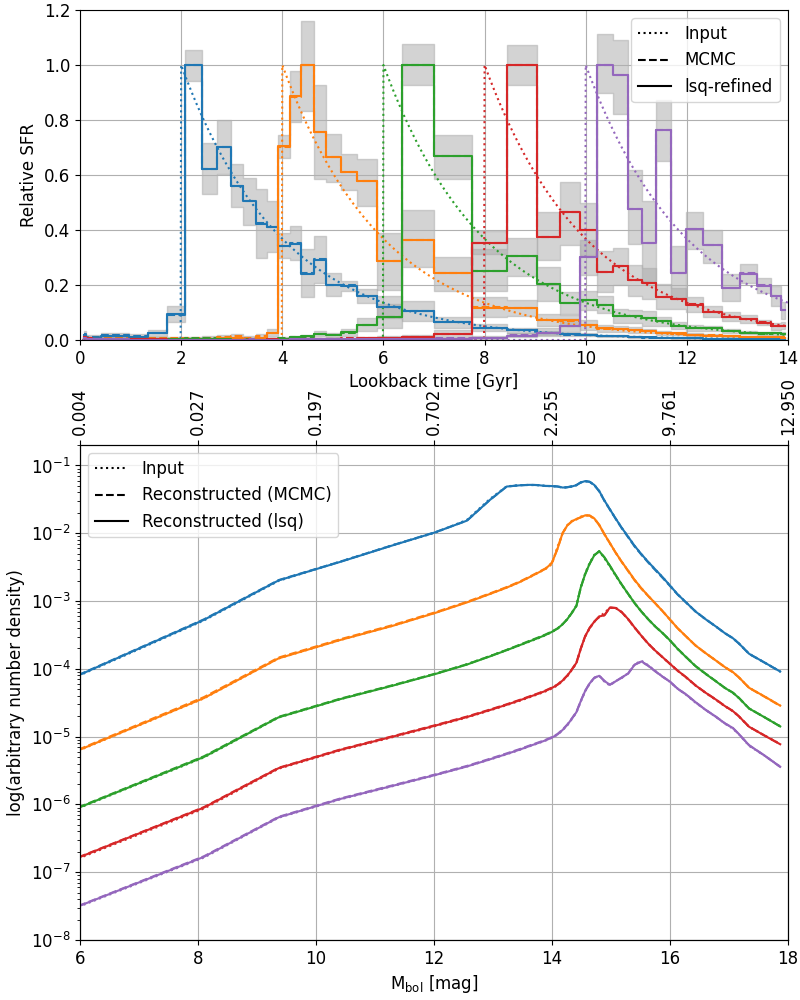
\includegraphics[width=\columnwidth]{figures/fig_01_exponential_decay_wdlf.png}
  \caption{Top: the recovered SFH and reconstructed SFH of a set of mock stellar
  populations with exponentially increasing star formation rates. Each of
  the population has an exponential constant of 3\,Gyr, the SFHs were truncated
  at a look-back time of 2, 4, 6, 8, and 10\,Gyr. See 
  Section~\ref{sec:magnitude_bin_size} for the explanation for the varying bin
  size in the lookback time. Middle: the input SFHs are plotted with dotted
  line; the marginalized results from the MCMC are plotted with dashed line;
  and the refined solutions with a least-square minimization method using a set
  of perturbed MCMC results as initial conditions are plotted in solid lines.
  The least-square method is to validate that the solutions are not trapped
  inside a local minimum. The last two are almost identical.}
  \label{fig:exponential_sfh}
\end{figure}

%%%%%%%%%%%%%%%%%%%%%%%%%%%%%%%%%%%%%%%%%%%%%%%%%%%%%%%%%%%%%%%%%%%%%%%%%%%%%%%%
\subsubsection*{Multiple bursts}
This set of WDLFs demonstrates that the method can retrieve sharp and
broad features whether they are distinctly separated or directly on top of each
other. The last set which comprises of all five sharp peaks and the broad
feature. It shows that there is some correlated results that are not completely
accounted for at around $6-7$\,mag. This is coming from the fact that the
pWDLFs are very similar as the WDLFs evolve the slowest at these magnitudes as
is obvious from the green and red curves in Fig.~\ref{fig:bursts_sfh}. We plan
to address this issue in future work by considering the colour
information~(see \ref{sec:conclusion}) which should relieve some degeneracy in
the solutions.

\begin{figure}
  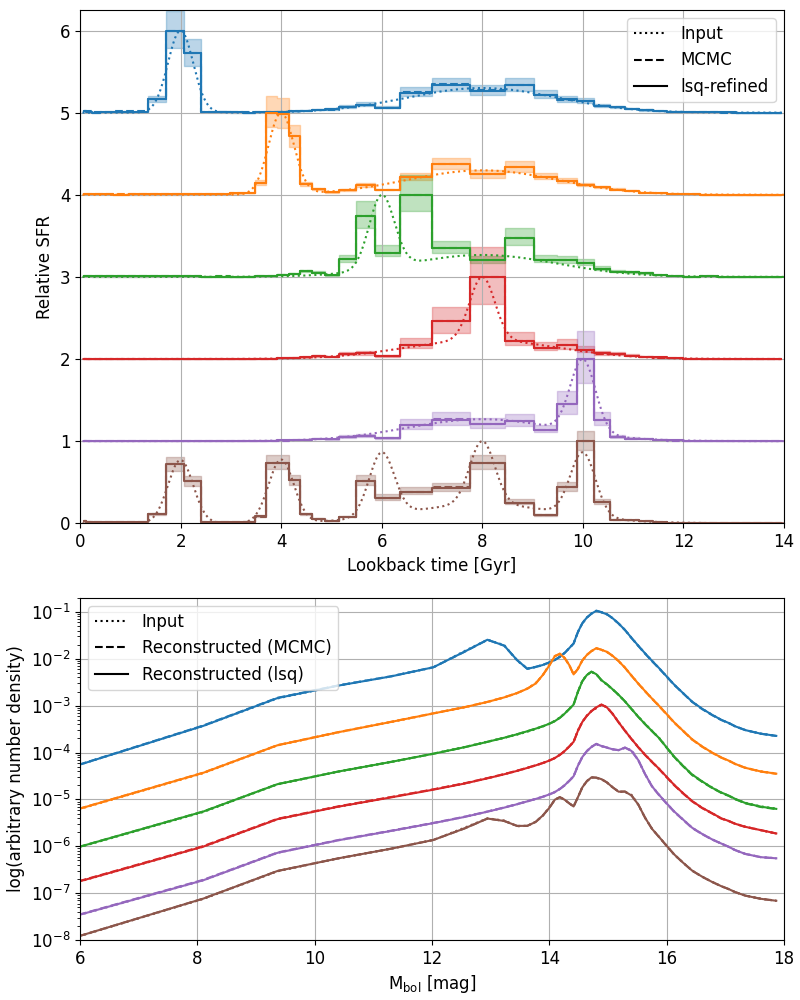
\includegraphics[width=\columnwidth]{figures/fig_02_two_bursts_wdlf.png} 
  \caption{The recovered SFH and reconstructed SFH of a set of mock stellar
  populations with a dual-burst SFH, and the second set has an inverse profile
  of the first set. (See Figure~\ref{fig:bursts_sfh}) for the legends.}
  \label{fig:bursts_sfh}
\end{figure}


%%%%%%%%%%%%%%%%%%%%%%%%%%%%%%%%%%%%%%%%%%%%%%%%%%%%%%%%%%%%%%%%%%%%%%%%%%%%%%%%
\section{Application to the Early Gaia Data Release 3}
\label{sec:application}
Upon deriving an SFH from a WDLF, one of the most important unsolved problems
is ``How much information can we obtain?''. We address in this work how, as a
first step, to achieve the maximal sampling in the magnitude space to extract
as much information from a WDLF as possible while avoiding the amplification of
noise. Any attempt to retrieve a signal at finer intervals than the
resolution of the data is essentially amplifying random noise. In this section,
we define the optimal bin sizes in bolometric magnitude, and how this naturally
defines the lookback time bin sizes.

\subsection{WDs from the GCNS}
%%%%%%%%%%%%%%%%%%%%%%%%%%%%%%%%%%%%%%%%%%%%%%%%%%%%%%%%%%%%%%%%%%%%%%%%%%%%%%%%
The GCNS contains 21\,848 WDs within a 100\,pc distance from us. The most
significant limitation from this sample is the uncorrected incompleteness. The
incompleteness is primarily at the bright end where there are very few WDs, and
in the faintest absolute magnitudes where the astrometric solutions are the
least reliable due the intrinsic faintness of these WDs. Furthermore, bright
WDs are rare, they are found only at larger distances, there are very few of
them in the local 100\,PC. The WDs were fitted with the pure hydrogen model from
the Montreal group~\citep{2019ApJ...876...67B} ignoring the effects of varying
the H/He atmospheric composition and surface gravity. They interpolated the
model grid to look up $G$-band bolometric corrections as a function
of ($G - G_{\mathrm{RP}}$) to map M$_\mathrm{G}$ to M$_{\mathrm{bol}}$ at
a fixed surface gravity of $\log(g)=8.0$. Because of the different colour
evolution as a function of the chemistry of the atmosphere, opting to fit a
pure hydrogen atmosphere limits the accuracy of the estimation of the cooling
ages as mixed hydrogen-helium atmosphere models give a shorter cooling age than
the pure hydrogen model does model~\citep{2022ApJ...934...36B}. 

When computing the WDLF, the GCNS adopted a fixed scaleheight of 365\,pc as
found from the GCNS itself. This choice can lead to significant effect on the
volumetric correction based on the 1/V$_{\mathrm{max}}$ method for deriving the
WDLF. Particularly, the scaleheight is increasing with time. However, such
evolution is never studied with a completeness corrected sample of
WDs~\citep{2006AJ....131..571H}, and previous works on empirical WDLFs all
adopted a fixed scaleheight~\citep{2006AJ....131..571H, 2011MNRAS.417...93R,
2019MNRAS.482..715L}.

This sample also assumed all WDs have come from isolated stellar evolution,
which would be a good assumption given that their colour-absolute magnitude
selection and the probability map in the colour-magnitude would have removed
WDs at unusually small and large surface gravities. These outliers are products
of stars that had gone through stellar interactions in the progenitor
systems~\citep[e.g.\ ][]{2013A&ARv..21...59I, 2023arXiv231117145H}.

The data product of the GCNS WDLF is a catalogue of WDs where each row
contributes $1\%$ to the WDLF: each WD has a posterior distribution in the
distance computation where each row has a solution of the maximum volume based
on the distance at that percentile. This is computed for the central $99$
percentiles of each WDs. In some cases the tail of the distribution exceeds
100\,pc, these WDs only have fractional contribution to the total WDLF. The
density normalization and the uncertainties in the WDLF have to be rescaled
properly when summing for the total WDLF because directly adding the solution
from each row will lead to an amplification of $\sim$$100$ times in the density
and similarly, the error bars would be $100$ times too small. Since the
catalogue has retained enough information on the bolometric magnitude and
distance, we can choose any bin size to present the GCNS WDLF as it is necessary
to optimally extracting the SFH. However, one down side of the catalogue is that
it does not come with the uncertainties of the derived bolometric magnitude so
we also refit the photometry that has taken into account of the photometric and
parallactic uncertainties, intrinsic distribution in the surface gravity and
the accuracy in using synthetic photometry~(see below).

%%%%%%%%%%%%%%%%%%%%%%%%%%%%%%%%%%%%%%%%%%%%%%%%%%%%%%%%%%%%%%%%%%%%%%%%%%%%%%%%
\subsection{Bin size}
\label{sec:magnitude_bin_size}
From the uncertainties in the photometric fitting for the bolometric magnitudes,
we can determine the resolution with which we can sample the WDLF. At the Nyquist
sampling rate~\citep{1949IEEEP..37...10S}, there should be two sampling points
in the space of one full-width at half maximum~(FWHM). Assuming the noise is
Gaussian, one FWHM is equivalent to $2.355$ standard deviations ($\sigma$).
Thus, the optimal sampling rate is $1.1775\sigma$ at the given magnitude.

%%%%%%%%%%%%%%%%%%%%%%%%%%%%%%%%%%%%%%%%%%%%%%%%%%%%%%%%%%%%%%%%%%%%%%%%%%%%%%%%
\subsubsection{Bolometric magnitude}
We have identified four main contributions to the uncertainties in the
bolometric magnitudes, with which we require to derive the size of the
smoothing kernel as a function of the bolometric magnitude.

\paragraph{Propagation of uncertainties \hfill\\}
\label{sec:propagation}
The propagation of uncertainties from the photometric and parallactic
measurements to the bolometric magnitude, either estimated from the minimization
function or an MCMC walk, are important contributors to the smoothing kernel,
but they do not directly correspond to the kernel.

\paragraph{Uncertainties in the synthetic photometry \hfill\\}
\label{sec:synthetic_photometry}
The synthetic photometry also comes with uncertainties, we estimate the model
uncertainty using the FWHM of the residuals in the SDSS filters reported in
\citet{2006AJ....132.1221H}. We take the mean FWHM of in $u$, $g$ and $r$ as
the proxy of $G_{\mathrm{BP}}$; the mean FWHM of $u$, $g$, $r$, $i$ and $z$
as a proxy of $G$; and the mean FWHM of $r$, $i$ and $z$ as the proxy of
$G_{\mathrm{RP}}$. Dividing them by $2.355$ gives us the dispersion that is
added to the Gaia magnitude uncertainty in quadrature. These values are found
to be $\sigma_{G_{\mathrm{BP}}}=0.0529$,
$\sigma_{G}=0.0462$ and $\sigma_{G_{\mathrm{RP}}}=0.0343$\,mag.

\paragraph{Intrinsic distribution of surface gravity \hfill\\}
\label{sec:logg_intrinsic_dispersion}
Singly evolved WDs follow a narrow distribution of surface gravity with
$\log(g)=7.998 \pm 0.011$ for DA~\citep{2021MNRAS.507.4646K}. An assumption
of a fixed surface gravity will lead to a small contribution to the smoothing
kernel as it increases the uncertainty.

\paragraph{Uncertainties in photometric fitting \hfill\\}
\label{sec:logg_photometric_fitting}
\citet{2014ApJ...796..128G} reported that photometric fitting with a model
grid of synthetic photometry leads to a dispersion of
$\sigma_{\mathrm{log}_{g}} = 0.404$ in the $\log(g)$, which is the combined
effect of the intrinsic dispersion and the precision. This is the quantity
required in this work because the GCNS sample of WDs was fitted assuming
a fixed surface gravity.

\paragraph*{Total uncertainties and dispersion \hfill\\}
In order to obtain the estimates of the uncertainties in the fitted bolometric
magnitudes due to the assumption of fixed surface gravity. We used
\textsc{WDPhotTools} to fit the GCNS WD samples in the three Gaia filters at
seven surface gravities. These seven values range from
$\log(g) - 3\sigma_{\mathrm{log}_{g}}$ to $\log(g) + 3\sigma_{\mathrm{log}_{g}}$
in an increment of one $\sigma_{\mathrm{log}_{g}}$. The photometric
uncertainties in the $Gaia$ filters are the sum in quadrature of the given
uncertainties in the photometry in each filter and the corresponding
uncertainties in the synthetic photometry~(Section \ref{sec:propagation} and
\ref{sec:synthetic_photometry}). While the $\sigma_{\mathrm{log}_{g}}$ is the
sum in quadrature of the intrinsic distribution of surface gravity and the
dispersion in surface gravity coming from photometric fitting~
(Section~\ref{sec:logg_intrinsic_dispersion} and \ref{sec:logg_photometric_fitting}).

From the seven fitted
bolometric magnitudes, we can approximate the dispersion with:
\begin{equation}
  \sigma_{M_{\mathrm{bol}}} = \frac{1}{6}\sum_{-3 \leq i \leq 3, i \neq 0}\frac{M_{\mathrm{bol}}(7.998 + i\sigma_{\mathrm{log}_{g}})}{|i|} - M_{\mathrm{bol}}(7.998)
\end{equation}
.

The Gaussian smoothing kernel is described by the sum of the fitting
uncertainties, the model uncertainties and the distribution coming from the
assumption of fixed surface gravity in quadrature~(blue scattered points in top
panel of Fig.~\ref{fig:magnitude_resolution}). The weighted average uncertainty
as a function of the bolometric magnitude is computed using the inverse maximum
volume as weights as it is used to weight each data point to the WDLF\footnote{
the bin centres of the bolometric magnitude used to compute the average are
1.5,  2.5,  3.5,  4.5,  5.25,  5.75,  6.25,  6.625, 6.85 to 17.25 in increment
of 0.2 and the last bin is centred at 17.475}.

%%%%%%%%%%%%%%%%%%%%%%%%%%%%%%%%%%%%%%%%%%%%%%%%%%%%%%%%%%%%%%%%%%%%%%%%%%%%%%%%
The use of WDLF relies on the assumption that WD shares similar properties
at the same luminosity. Based on such an underlying assumption, we measure
the mean of these dispersions weighted by the $1/\mathrm{V}_{\mathrm{max}}$
as provided in the GCNS WD catalogue. Then they are fitted with a spline as
a function of bolometric magnitudes~(see Fig.~\ref{fig:magnitude_resolution}
and Table~\ref{tab:magnitude_resolution} in the appendix for the interpolation
presented in the middle panel of Fig.~\ref{fig:magnitude_resolution}) to get
the average uncertainty as a function of the bolometric magnitude.

%%%%%%%%%%%%%%%%%%%%%%%%%%%%%%%%%%%%%%%%%%%%%%%%%%%%%%%%%%%%%%%%%%%%%%%%%%%%%%%%
\subsubsection{Lookback time}
The WDLFs with short bursts of star formation are strongly peaked at a single
magnitude (see, for example, the set of pWDLFs in Fig.~\ref{fig:basis_pwdlf}).
Thus, adding the monotonically cooling nature of WDs, there is a one-to-one
mapping of the cooling age of the population and the peak magnitude (see middle
panel of Fig.~\ref{fig:magnitude_resolution}. Although at older ages, with the
peak magnitude beyond $15$\,mag, a WDLF starts to show double peaks, there is
always a dominant peak that is at least half an order of magnitude higher in
the number density. Thus, we can reliably relate the two relations: peak
magnitude--age and peak magnitude--magnitude-resolution. Where the magnitude
has a one-to-one mapping to the age of the system, we can obtain the time
resolution in which we construct the set of the basis pWDLFs that would allow
the extraction of the SFH at the maximum sampling rate (i.e.\ the minimum bin
size) without the amplification of noise.

%%%%%%%%%%%%%%%%%%%%%%%%%%%%%%%%%%%%%%%%%%%%%%%%%%%%%%%%%%%%%%%%%%%%%%%%%%%%%%%%
At the oldest age~(i.e.\ faintest magnitudes), the uncertainties of the
bolometric magnitude is most likely underestimated as the value
$\sigma_{\mathrm{log}_{g}} = 0.404$ from \citet{2014ApJ...796..128G} did not
include WDs from the faint end. Additionally, from the recent calibration
works~(Bergeron), it is known that the models are less accurate at the lowest 
temperature, and the bolometric magnitudes obtained by assuming DA or DB
atmosphere are fainter than what mixed hydrogen-helium models would
give~\citep{2022ApJ...934...36B}. However, we cannot quantify these uncertainties
so we only caution readers to pay attention is drawing conclusions from any
information fainter than $\approx15.5$\,mag, which corresponds to a look back
time of $\approx9$\,Gyr.

%%%%%%%%%%%%%%%%%%%%%%%%%%%%%%%%%%%%%%%%%%%%%%%%%%%%%%%%%%%%%%%%%%%%%%%%%%%%%%%%
\begin{figure}
    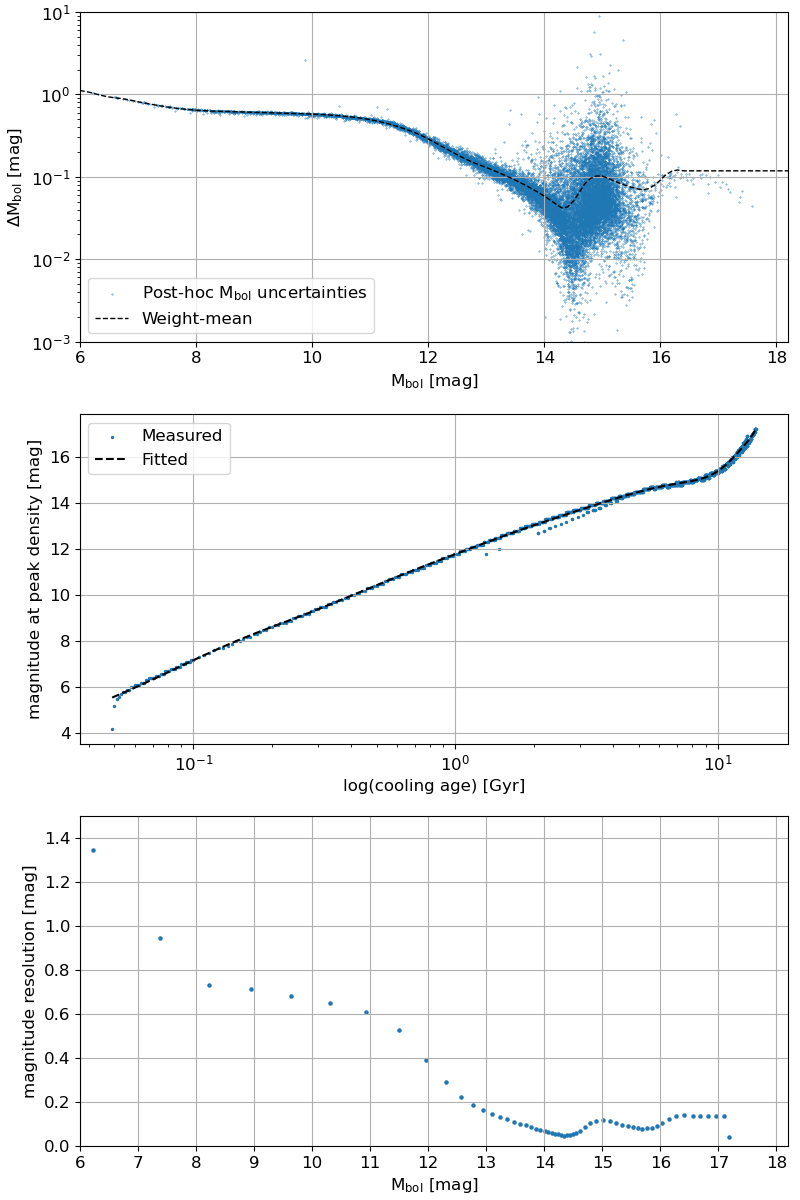
\includegraphics[width=\columnwidth]{figures/fig_03_mbol_sigma_magnitude_resoltuion.png}
    \caption{Top: the total uncertainties in the bolometric magnitude as a 
    function of bolometric magnitude~(blue). Due to the small
    number of data points, the weighted average at magnitudes fainter than
    $16.5$\,mag are not computed. At these magnitudes, the uncertainties at the
    last bin centred at $16.45$\,mag is used. Middle: the bolometric magnitude
    at which the peaks of the pWDLF are located. Bottom: the bolometric
    magnitude resolution of the WDLF computed using the fitting uncertainties
    from the top figure and the added uncertainties coming from the synthetic
    photometry and the assumption of fixed surface gravity~(see text). The
    low resolution in the bright end comes from a combination of large
    uncertainties in the observed magnitudes, the lack of UV photometry and the
    sensitivity of the solution to the surface gravity.}
    \label{fig:magnitude_resolution}
\end{figure}

%%%%%%%%%%%%%%%%%%%%%%%%%%%%%%%%%%%%%%%%%%%%%%%%%%%%%%%%%%%%%%%%%%%%%%%%%%%%%%%%
\begin{figure}
    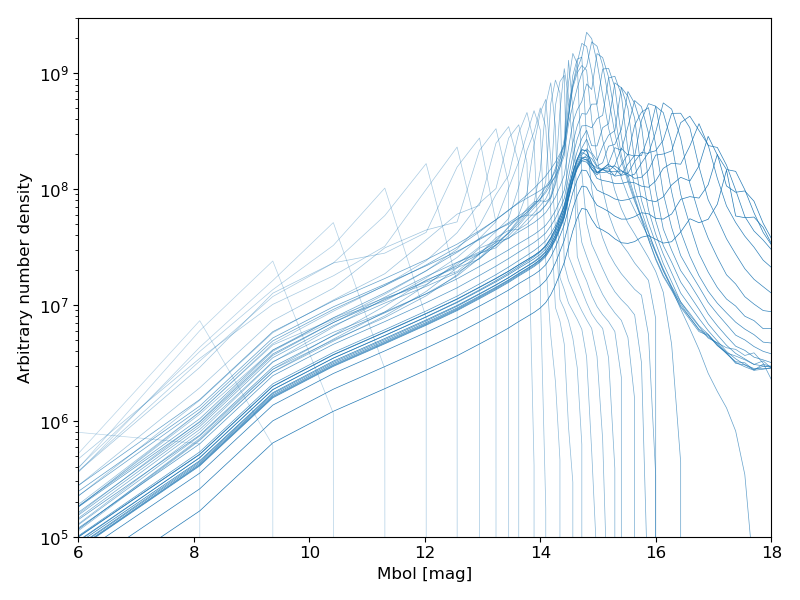
\includegraphics[width=\columnwidth]{figures/fig_04_basis_pwdlf.png}
    \caption{The set of partial WDLF (basis functions) that the peaks are
    separated by the magnitude resolution as found in
    Fig~\ref{fig:magnitude_resolution}. At older ages, double peaks start to
    emerge. However, there is always a dominant peak that is at least half an
    order of magnitude higher in the contribution.}
    \label{fig:basis_pwdlf}
\end{figure}

%%%%%%%%%%%%%%%%%%%%%%%%%%%%%%%%%%%%%%%%%%%%%%%%%%%%%%%%%%%%%%%%%%%%%%%%%%%%%%%%
\subsection{Star Formation History}

By applying the set of basis functions to the fitting method as described in
section \textsection\ref{sec:model_fitting}, because the set of pWDLFs is
normalised the same way, the relative contribution translates to the relative
SFH of the solar neighbourhood. The absolute normalisation can be found by
matching the reconstructed WDLF to the integrated number density of the input
WDLF, and correct for the irregular bin size. We have found multiple phases of
enhanced star formation using this novel method, these bursts and lulls are all
in good agreement with previous works found using other methods and stellar 
popluations~(see Fig.~\ref{fig:sfh_optimal} and the next section). We find a
strong burst of star formation at $\sim$3\,Gyr, and some prominent enhanced
star formation at $\sim$2, 4, 9 and 11\,Gyr~(see bottom panel of
Fig.~\ref{fig:sfh_optimal})

%%%%%%%%%%%%%%%%%%%%%%%%%%%%%%%%%%%%%%%%%%%%%%%%%%%%%%%%%%%%%%%%%%%%%%%%%%%%%%%%
The 20\,pc subset\ shows the contribution of the
WDs within the 20\,pc distance, it should \textit{not} be interpreted as a
20\,pc sample where the maximum volume (upper integral limit) for each WD would
be different to that of a 100\,pc sample, hence we have opted for the word
``subset''. We show this subset for the purpose of a more meaningful comparison
of other works that probed much smaller volumes~(see 
Section~\ref{sec:comparison}). As already pointed out in the previous section,
we caution readers to pay particular attention in drawing conclusions from any 
information older than $\sim$$9$\,Gyr due to, most likely, some correlated
signals unaccounted for.

\begin{figure}
    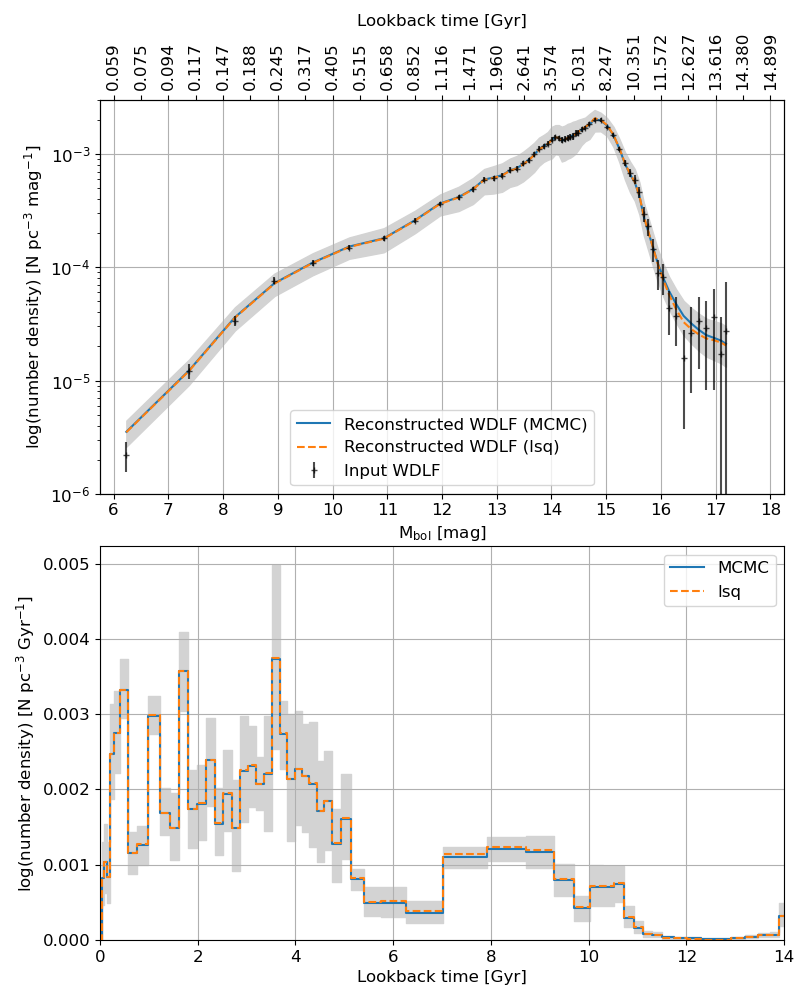
\includegraphics[width=
    \columnwidth]{figures/fig_05_gcns_reconstructed_wdlf_optimal_resolution_bin_optimal.png}
    \caption{Top: the reconstructed WDLF using the pWDLFs, the set of solutions
    refined with a least square method shows marginal improvement. The 20\,pc
    subset shows the contribution of the WDs within the 20\,pc distance, it
    should \textit{not} be interpreted as a 20\,pc sample. The x-axis on
    the top side shows only the cooling age WDs but not the total age. A
    luminosity function has marginalised over the progenitor masses, so the total
    age of WDs is not linearly mapped to the axis of this figure. Bottom: The
    weights of the pWDLFs transformed to the unit of per billion year by dividing
    by the bin widths, and by normalising with the number density to get the
    unit of per cubic parsec. The raw weights are found from MCMC sampling
    and finishing with a least-squares minimisation.}
    \label{fig:sfh_optimal}
\end{figure}


%%%%%%%%%%%%%%%%%%%%%%%%%%%%%%%%%%%%%%%%%%%%%%%%%%%%%%%%%%%%%%%%%%%%%%%%%%%%%%%%
\section{Comparison and discussion}
\label{sec:comparison}

\subsection{WDLF}
\label{sec:inversion}
%%%%%%%%%%%%%%%%%%%%%%%%%%%%%%%%%%%%%%%%%%%%%%%%%%%%%%%%%%%%%%%%%%%%%%%%%%%%%%%%
In order to validate the results in this paper, we have compared the
resulting star formation history with the equivalent result obtained from an
independent method applied to the same input WDLF.

%%%%%%%%%%%%%%%%%%%%%%%%%%%%%%%%%%%%%%%%%%%%%%%%%%%%%%%%%%%%%%%%%%%%%%%%%%%%%%%%
\citet{2013MNRAS.434.1549R} presented a method to estimate the star formation
history from WDLFs using an inversion algorithm on the integral 
Equation~\ref{eqn:wdlf}. Their method is based on the expectation-maximization
algorithm similar in principle to the Richardson-Lucy deconvolution, which is
used to obtain maximum-likelihood solutions to inverse problems in the presence 
of missing data -- which in the present application is the unknown distribution
of WD mass as a function of magnitude.

They have recently updated the inversion algorithm........

They have applied this new algorithm using an identical set of models to the
GCNS dataset and have independently computed the SFH as shown in
Figure~\ref{fig:nr_sfr}, with the accompanying reconstructed WDLF and residuals
shown in Figure~\ref{fig:nr_wdlf}.


\begin{figure}
    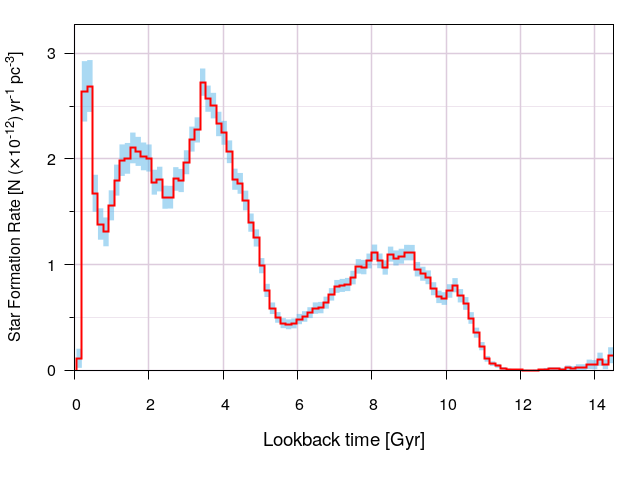
\includegraphics[width=\columnwidth]{figures/nr_sfr.png}
    \caption{Star formation rate obtained by inversion of the GCNS WDLF using the
    algorithm presented in \citet{2013MNRAS.434.1549R} and described in 
    section~\ref{sec:inversion}.}
    \label{fig:nr_sfr}
\end{figure}

\begin{figure}
    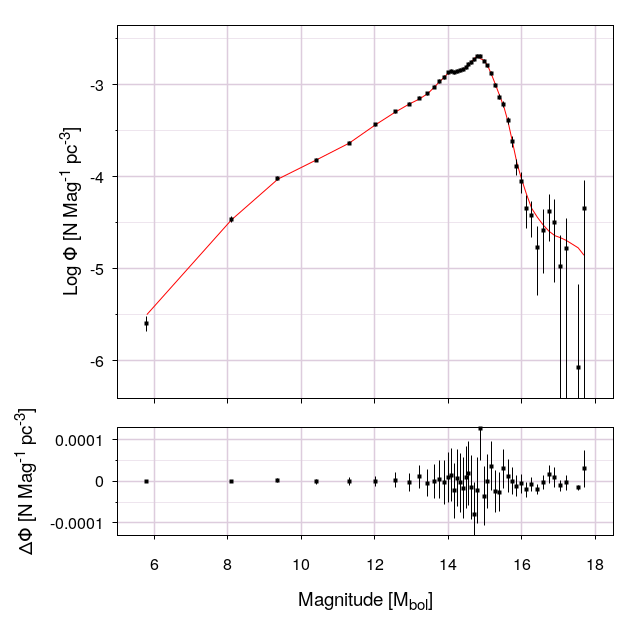
\includegraphics[width=\columnwidth]{figures/nr_wdlf.png}
    \caption{Comparison between the observed (black points) and model (red line)
    WDLF obtained from the inversion algorithm, and corresponding to the star
    formation history presented in figure~\ref{fig:nr_sfr}.}
    \label{fig:nr_wdlf}
\end{figure}

%%%%%%%%%%%%%%%%%%%%%%%%%%%%%%%%%%%%%%%%%%%%%%%%%%%%%%%%%%%%%%%%%%%%%%%%%%%%%%%%


\subsection{Other methods using WDs}
%%%%%%%%%%%%%%%%%%%%%%%%%%%%%%%%%%%%%%%%%%%%%%%%%%%%%%%%%%%%%%%%%%%%%%%%%%%%%%%%
\textit{T14} reported the SFH using a 20\,pc volume-complete sample. They found roughly
two broad bursts of SFH with a higher intensity in the recent 5\,Gyr peaking at
3.5\,Gyr and a lower step between 5 and 12\,Gyr with a peak at 8.5\,Gyr. They
are reporting the SFH by means of the direct number count of WDs hence further
bias corrections are required. These main-sequence bias as termed in T14 
is already handled when constructing the WDLF in our case. The kinematics bias
is uncorrected in the GCNS sample, and we have not attempted to correct it
because in order to perform the correction properly, it has to be computed 
together in the integral of the maximum volume~\citep{2015MNRAS.450.4098L}.
Nevertheless, for a sample that does not require stringent selection
criteria, for example, when studying high-velocity WDs only, the
kinematic correction is small.

Based on a comparison between T14 and R13, they pointed out a concern regarding
the methods of mathematical inversion in the application SFH retrieval from a
WDLF. We have shown in Fig.~\ref{fig:sfh_optimal} the contribution of SFH
from the WDs within a distance of 20\,pc that the peak of star formation at a
lookback time of about 0.3\,Gyr is almost completely disappeared and the SFH is
dominated by the broad peak centered at just under 4\,Gyr, which is in good
agreement with T14. A second broad feature between 8 and 12\,Gyr with a sharp
peak at 11\,Gyr has some resemblance to their findings. The differences, which
is mostly a translation and scaling in the direction of the lookback time, is
likely to be coming from the adoption of different cooling models. 
\citet{2022RASTI...1...81L} has illustrated the effect of various models on 
the shape of the WDLFs. Model combinations C \& D in Figure~12 of their work show how the 
switching between the cooling models including phase separation can lead to
a 0.5\,mag difference in the position where WDs pile up (due to significant
slowdown of the cooling). From Fig.~\ref{fig:sfh_optimal}, it is clear from the
top axis that at these magnitudes, the cooling age is very sensitive to the
bolometric magnitude between 13 and 16\,mag, corresponding to a cooling age of
1.25 and 9.76\,Gyr, respectively, at the two limits.

%%%%%%%%%%%%%%%%%%%%%%%%%%%%%%%%%%%%%%%%%%%%%%%%%%%%%%%%%%%%%%%%%%%%%%%%%%%%%%%%
%\citet{2019ApJ...887..148F} computed the SFH from a deep proper motion survey,
%however, their sample is only corrected for photometric incompleteness. The
%untreated kinematic bias can lead to incompleteness in the sample
%selection~\citep{2014ApJ...791...92T, 2015MNRAS.450.4098L}. Nevertheless, this
%bias is unlikely to have a large impact on the thin disk population, yet in
%their recovered SFH, a nearly-constant SFH was found. It brings up two immediate
%questions: (1) is the recent burst that is seen in a few other works direction-
%dependent? and (2) does the recent burst attributed to any major streaming that
%occupies a different part of the velocity space? These are important
%questions to be addressed in future works.

% I am unable to recreate their plots with the values reported in their work.

%%%%%%%%%%%%%%%%%%%%%%%%%%%%%%%%%%%%%%%%%%%%%%%%%%%%%%%%%%%%%%%%%%%%%%%%%%%%%%%%
\textit{C23} made use of a similar sample to this work, they found a constant
star formation rate over the last 10.5\,Gyr with the 40\,pc sample of WDs.
It is a simple flat line of a top hat function. Their recovery method overlooks
methods available to more optimally extracting information from a given
signal~(as we described in details in \ref{sec:magnitude_bin_size}). It is 
possible to identify an optimal bin size and the set of bin sizes determines
the time resolution in which we can derive the SFH. In observation astronomy,
using photometry as an example, optimal extraction based on a known
point-spread function is a technique to maximise the signal-to-noise ratio in
the photometry~\citep{1980SPIE..264..171T, 1987PASP...99..191S}. It is possible
because we have information on how a point appears on the detector plane after 
going through the optical system from the telescope mirror~(or even to model
the Earth's atmosphere if adaptive optics is used) to the detector plane. Very 
similar reasoning is used in, and not limited to, image differencing where a
point spread function is used~\citep{1998ApJ...503..325A, 2008MNRAS.386L..77B, 
2009MNRAS.397.2099A, 2016ApJ...830...27Z}, spectroscopy using a line spread
function~\citep{1986PASP...98..609H, 1989PASP..101.1032M, 2003PASP..115..688K},
image reconstruction where the smoother kernel is
known~\citep{1972JOSA...62...55R, 1974AJ.....79..745L}, and image
deconfusion where the position of two confused sources are known from an
external source~\citep{2015A&A...582A..15M}.

%%%%%%%%%%%%%%%%%%%%%%%%%%%%%%%%%%%%%%%%%%%%%%%%%%%%%%%%%%%%%%%%%%%%%%%%%%%%%%%%
Secondly, we attribute the main differences in our derived SFH to their
use of chi-squared statistics in fitting cumulative distribution
functions~(CDF). By fitting a CDF directly to the cumulative data, one would
run into significant issues coming from strongly correlated values in the
neighbouring values in the ordinal axis. The uncertainty of a data point on
a CDF is not merely the uncertainty in that given bin, the uncertainties
accumulate to the successive bins non-linearly, depending on how accurate the
measurement can be made on the observed variable. In this case, the measurement is the absolute
magnitude in the $G$ band. A Poisson error can serve as the lower limit of
the uncertainties at best. Specific to fitting a CDF of the bolometric
magnitude of WDs, the faintest WDs are most poorly determined because of both
uncertainties in the measurement and those in the models. Fitting such CDF
with a $\chi^2$-minimisation method is significantly putting too much weights
on the least reliable data. Specifically, the faintest WD has a perfect
measurement because that is when the CDF has to converge to unity.

%%%%%%%%%%%%%%%%%%%%%%%%%%%%%%%%%%%%%%%%%%%%%%%%%%%%%%%%%%%%%%%%%%%%%%%%%%%%%%%%
Thirdly, the scale height they have adopted~(75\,pc) is much smaller than those
adopted by all other WDLF works~(e.g.\,\citealt{2006AJ....131..571H,
2011MNRAS.417...93R, 2019MNRAS.482..715L}). Particularly,
\citet{2006AJ....131..571H} found that the typical minimum and maximum scale
height of WD at different bolometric magnitudes span between 200 and 900\,pc.
C23's choice of scaleheight is coming from young open clusters, which is not
a representative population for the evolution of the galaxy. Given these open
clusters remain open clusters by their self-gravity, this value can, at best,
set the lower limit of the scaleheight as the progenitor clusters had to have
dissolved by the time we observe these isolated WDs. We agree that the youngest
WDs should have a smaller scaleheight, and both the scaleheight and
$\sigma_W$~(velocity dispersion perpendicular to the Galactic plane) increase
with time. However, assuming both functions increase linearly with time as
adopted in their work, the gradients of the two relations are not the same,
doubling in $\sigma_W$ from 1 to 8\,Gyr~(Fig.~4 in their work) does not mean
the scaleheight doubles over the same time. There is a missing multiplier
that should be at least a factor of $\sim$2 to $\sim$3 judging from how the
aforementioned works found a typical scale height of $\sim$300\,pc. The
effect of this missing factor in a simulated population of WDs should lead to
an over-density of the older WDs. This can explain the consistent trend of 
deviation starting at the brightest WD up to $\sim$13\,mag~(cooling time of
$\sim$1\,Gyr) because the effect is strongest for the youngest WDs where the
scaleheight is comparable to the distance limit of 40\,pc, particularly with 
there is an offset of 20\,pc of the Sun from the Galactic plane. Furthermore,
as the boundary conditions of fitting CDF, the residual converges to 0.0 at the
brightest and faintest magnitudes. One should not read it as proof of the
quality of the fit. As a consequence of such a requirement, the most effective
way is to fix the overdensity is to, numerically, reduce the SFH, hence a
truncation in the SFH can lead to the modelled CDF constantly smaller than the
40\,pc sample.

%The reason they observe little change in the 2-part and 3-part
%SFH because the number density of a WDLF is highest at $\sim$15\,mag, which
%requires WDs at least 7\,Gyr in cooling age 

%%%%%%%%%%%%%%%%%%%%%%%%%%%%%%%%%%%%%%%%%%%%%%%%%%%%%%%%%%%%%%%%%%%%%%%%%%%%%%%%
\textit{\citet{2019ApJ...878L..11I}} performed an analysis by directly
computing the star formation history of a population of massive WDs selected
from \citet{2019Natur.565..202T}. The choice of using only massive WDs
removes the degeneracy issues given rise from the choice of metallicity models
of the progenitors; and the fact that massive WDs are remnants of the most
massive stars that could have turned into WDs where their progenitor lifetime
is short compared to the WD cooling age. They found an abrupt start of star
formation at $\sim$7\,Gyr and an enhanced star formation around 2-3\,Gyr. They
also note that they find a burst at $\sim$0.4\,Gyr when applying their method
on the 25\,pc sample from~\citet{2017ASPC..509...59O}. This recent burst was not
seen in all but one previous work -- R13's. Interestingly enough, we have
recovered the same peak with the GCNS sample using the improved-R13 inverse
modelling method (Section~\ref{sec:inversion}) and the pWDLF forward modelling
method~(this work). 

%%%%%%%%%%%%%%%%%%%%%%%%%%%%%%%%%%%%%%%%%%%%%%%%%%%%%%%%%%%%%%%%%%%%%%%%%%%%%%%%
\textit{\citet{2021MNRAS.502.1753T}} analysed a 100\,pc sample WDs from
Torres et al.~(2019) with a completeness of $91\%$ at 20.5\,mag. This sample
contains 95 WDs that are disentangled into thin disk, thick disk and stellar
halo components. The data with their selection criteria applied is commonly
referred to as a high-velocity sample, but their treatment of the data
selection is much more sophisticated making use of a supervised
machine learning method based on Random Forest techniques in eight-dimensional
space. They found a cut-off age of $12\pm0.5$\,Gyr where the peak of star
formation happened at $\sim$11\,Gyr. The star formation continued for about
4\,Gyr. $13\%$ of their WDs are younger than 7\,Gyr which is puzzling given
their kinematic choice, spurious WDs from the thin and thick disk should not
have attributed to such a fraction of contamination. They suggested that
individual analysis will be required to unravel the origin of these objects.

%%%%%%%%%%%%%%%%%%%%%%%%%%%%%%%%%%%%%%%%%%%%%%%%%%%%%%%%%%%%%%%%%%%%%%%%%%%%%%%%
\subsection{MS stars}
There are a number of works concerning the SFH of the solar neighbourhood. We
have selected the following three because their sample selections are similar
to that of the GCNS sample with little directional dependence.

%%%%%%%%%%%%%%%%%%%%%%%%%%%%%%%%%%%%%%%%%%%%%%%%%%%%%%%%%%%%%%%%%%%%%%%%%%%%%%%%
\textit{\citet{2006A&A...459..783C}} used the $Hipparcos$ catalogue of stars
within 80\,PC of the Sun and brighter than $V=8$\,mag. The restrictive selection
has significantly excluded the effects due to photometric or kinematic
incompleteness. They computed the SFH by minimising the differences between the
colour-magnitude diagram of the population from the Hipparcos data and the
sum of the partial CMD~(the concept that inspired this work to use partial
WDLFs). They recovered the strongest star formation at a lookback time of
$\tau=2-3$\,Gyr, and a slowly decreasing SFH up to $\tau=6$\,Gyr where there is
a sharp drop in SFR until $\tau=10-12$\,Gyr. Their SFH shows excellent agreement
to our work, except for the strong peak at the most recent time~(see more in
Section~\ref{sec:conclusion}).

%%%%%%%%%%%%%%%%%%%%%%%%%%%%%%%%%%%%%%%%%%%%%%%%%%%%%%%%%%%%%%%%%%%%%%%%%%%%%%%%
\textit{\citet{2007ApJ...665..767R}} used the Hipparcos catalogue to calibrate
bias in the \citep{2005ApJS..159..141V} volume-limited spectroscopic
sample of 1\,039 FGK dwarfs in the solar neighbourhood with estimates of
their age and metallicity. They went through thorough selection criteria,
which resulted in two samples. Each sample has limiting absolute magnitudes
between $4$ and $\sim$6 mag, with a distance limit of $\sim$30\,PC, and MS mass
in the range $\sim1.25$ to $\sim0.8$\,M$_{\sun}$. Their results are a direct
number count of stars in a volume-limited survey that only include late F to
early K stars, so their SFH as plotted in Fig.~\ref{fig:comparison} is a simple
normalisation by multiplying by an arbitrary value to allow comparison of the
\textit{shape}, particularly the peaks and troughs of the SFH. The most notable
peaks from their work are at $2$ \& $4$\,Gyr. Two narrow peaks at $6$ \&
$8$\,Gyr are also present.

%%%%%%%%%%%%%%%%%%%%%%%%%%%%%%%%%%%%%%%%%%%%%%%%%%%%%%%%%%%%%%%%%%%%%%%%%%%%%%%%
\textit{\citet{2018IAUS..330..148B}} used the TGAS data to perform an initial
analysis with the technique of synthetic colour-magnitude diagram-fitting, they
found a recent star burst at a lookback time of $\sim$2--3\,Gyr, an enhanced
star formation $\sim$6--10\,Gyr. Figure~\ref{fig:comparison} shows their
\textit{mildly corrected} solutions.

%%%%%%%%%%%%%%%%%%%%%%%%%%%%%%%%%%%%%%%%%%%%%%%%%%%%%%%%%%%%%%%%%%%%%%%%%%%%%%%%
\textit{\citet{2019A&A...624L...1M}} selected from Gaia DR2 2\,890\,208 stars
with mean G$_{\mathrm{DR2}}<12$, estimated to be $97\%$ complete. Only stars
with proxy-absolute magnitude $G_{\pi}$ brighter than 10 mag are considered in
their second filtering in order to remove all brown dwarfs and white dwarfs in
their analysis. They applied a non-parametric method that uses an approximate
Bayesian computation~\citep{2017A&C....19...16J} algorithm to compute their
merit function by comparing the Gaia data against the Besancon Galaxy model
fast approximation simulations~\citep{2018A&A...620A..79M}). They have found
that their analysis is most affected by the thick disk modelling and the
stellar evolution models. From their four choices of fitting configurations of
the Gaia sample. They see a general trend of decreasing star formation from
$\sim$10\,Gyr to 6\,Gyr, followed by an enhanced star formation of 4\,Gyr in
duration with a peak at $\sim$2.5\,Gyr. They also found a sharp and fast drop
in the star formation rate in the most recent 1\,Gyr.

\subsection{Subgiants}
%%%%%%%%%%%%%%%%%%%%%%%%%%%%%%%%%%%%%%%%%%%%%%%%%%%%%%%%%%%%%%%%%%%%%%%%%%%%%%%%
\citet{2022Natur.603..599X} uses subgiants to map the metallicity, angular
momentum and SFH of the Milky Way. The distance they probe is much larger
than this work so it is expected that the recovered SFH show different
features. Nevertheless, they observe one dominant peak at 10.5\,Gyr and two
small peaks at 2 and 4\,Gyr.

\begin{figure}
  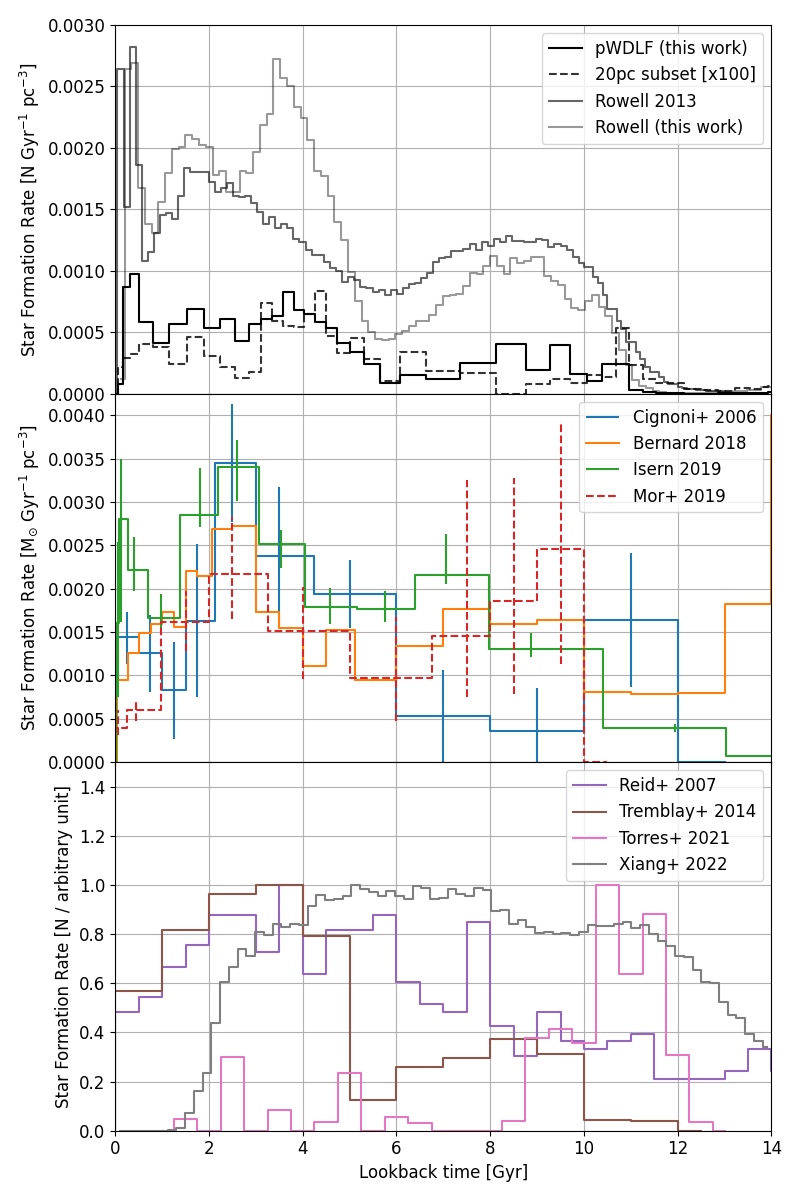
\includegraphics[width=\columnwidth]{figures/fig_08_compare_sfh.png}
  \caption{Comparision of the recovered SFH against previous works, see body
  text of Sec~\ref{sec:comparison} for details. Top: SFH retrieved with the
  pWDLF method, R13 results (with the H06 WDLF), and the SFH derived using the
  improved-R13 algorithm on the GCNS WDLF. The 20\,pc subset of the GCNS is
  also plotted for comparison~(see body text for details). The SFH is reported
  in the unit of number of stars formed per unit time per unit volume.
  Middle: The SFH using four independent methods and samples reported in the
  unit of solar mass formed per unit time per unit volume~(solid line) or
  projected-area~(dashed line). Bottom: The SFHs that are derived from four
  other independent methods and samples in the unit of number of stars formed
  per arbitrary time and spatial unit.}
  \label{fig:comparison}
\end{figure}

%%%%%%%%%%%%%%%%%%%%%%%%%%%%%%%%%%%%%%%%%%%%%%%%%%%%%%%%%%%%%%%%%%%%%%%%%%%%%%%%
\section{Conclusions and Future Work}
\label{sec:conclusion}
By properly propagating the uncertainties in the systematics and measurements,
this work has shown that it is possible to recover the star formation history 
using WDLF accompanied by meaningful uncertainties that encompass the 
uncertainties in the WD atmosphere models, the photometry and the consequence
of assuming a fixed surface gravity in the determination of the bolometric 
magnitude. Using the bin sizes that are representative of the data given the
known effect of how the uncertainties limit the resolution of the signal, we
have chosen a set of varying bin sizes such that it matches the Nyquist
sampling rate where two sampling points are required for every FWHM. It is 
obvious from our careful treatment of uncertainties, along with the comparison 
from other works, that with the currently available surveys and computing
facilities, we can retrieve complex signals from the given noisy data using
well-established mathematical tools and good knowledge of the optical system.
The recovered SFHs agree particularly well at an intermediate age of 1-8\,Gyr.
We outline the most imminent issues to be addressed as follows:

%%%%%%%%%%%%%%%%%%%%%%%%%%%%%%%%%%%%%%%%%%%%%%%%%%%%%%%%%%%%%%%%%%%%%%%%%%%%%%%%
\subsection*{List of Known issues}
\begin{enumerate}
    \item The GCNS sample is not incompleteness corrected, particularly, the
    kinematic selection can lead to a significant 
    bias~\citep{2014ApJ...791...92T, 2015MNRAS.450.4098L} in the analysis that
    leads to underestimation in the number densities. Although not applicable to the GCNS
    sample, the parallax-related selection usually lead to Lutz-Kelker 
    bias~\citep{1973PASP...85..573L}, which would affect the shape of the
    WDLF, hence the SFH.
    \item The model uncertainty in the synthetic photometry is considered,
    however, the treatment is not rigorous as the uncertainty should be as
    a function of the bolometric magnitude. Particularly, it is known that
    in the visible wavelengths, the errors are the largest at the coolest end.
    \item MS progenitors: the initial mass function, scaleheight evolution,
    metallicity evolution, initial-final mass relation, and the
    binary/multiplicity fraction can lead to bias in the derived WDLF. As
    noted by \citet{2019ApJ...878L..11I}, the R13 method is sensitive to the
    adopted metallicity and IMF models but not the DA/non-DA ratio and among
    other choices of models. Although the pWDLF method does not suffer similar
    convergence and regularisation issues, this method is also sensitive to
    the choice of MS models, as would any method that requires MS lifetimes
    in the analysis.
    \item WDs: the effects from the choice of cooling models, atmosphere
    models, synthetic photometric models, and unresolved binary WDs have to be
    taken into account.
    \item Completeness in the bright end: these hot WDs can be seen from the
    largest distance, so they should be the most complete in a 100\,pc
    sample. However, the single scaleheight of 250\,pc used in the entire
    sample of GCNS WDs can lead to a bias. Particularly, as pointed out in
    C23, the scaleheight of the youngest WDs could be
    as low as 75\,pc.
    \item Completeness in the faint end: Gaia has a detection limit of
    $\sim$20.5\,mag, at 100\,pc where the distance modulus is 5\,mag, an
    absolute magnitude of $\sim$15.5\,mag in $G$ is a naive derivation of the
    completeness limit.
    \item The sample size is large enough that we should investigate the
    directional dependency of the WDLFs, the CFHS survey seems to reveal a
    WDLF more dissimilar to the WDLFs from SDSS, SuperCOSMOS and Gaia.
    \item The distance dependency should be investigated as well, the shape of
    the SFHs from different works roughly agree to when the most recent strong
    star formation happened. However, the normalisation and the relative SFH
    vary quite strongly from work to work. This is likely due to not only the
    choice of stellar population being studied, but due to different
    contributions from different stellar populations as different works look
    into a different depth.
\end{enumerate}

%%%%%%%%%%%%%%%%%%%%%%%%%%%%%%%%%%%%%%%%%%%%%%%%%%%%%%%%%%%%%%%%%%%%%%%%%%%%%%%%
When comparing with the T14 sample, we realized that there is a striking 
difference in the SFH from the 20\,pc and 100\,pc sample at the most recent
time. This brings up three important points that should be investigated: first,
an arbitrary selection of SFH reported from different work cannot draw
meaningful comparison; second, even at the scale in the order of 10\,pc, we
can observe variations of SFH; third, if the SFH is a strong function of
distance from the Sun, then the directional dependency must be strong given the
Sun is not located in the middle of the Galactic plane, and it is not located
in a major arm of the Galaxy. The analysis should be more complex than simply
dividing the sample into zones of Galactic latitudes because, for example,
looking into the length of the Orion-Cygnus arm where the Sun resides, should
be different to looking into the inter-arm regions -- Perseus arm and
Carina-Sagittarius arms are too far away for WD studies, so looking into their
directions will only give us the WDs in the foreground.

As pointed out in \citet{2019A&A...624L...1M} and \citet{2019ApJ...878L..11I},
the decreasing SFR trend from $\sim$10 to 6\,Gyr is consistent with the
onset of quenching observed in a cosmological context at a redshift of
z$\sim$1.8~\citep[corresponds to a lookback time of
$\sim$10\,Gyr, e.g.][]{2016MNRAS.461.1100R, 2017MNRAS.471.4155K}. It is
also compatible with the evidence of the quenching of the Milky
Way~\citep{2016A&A...589A..66H}. This is in line with the thick-disc formation
scenario attributed to a major merger event at a lookback time of 
$\sim$10\,Gyr~\citep{2018Natur.563...85H}.

Beyond systematics and directional dependence, one obvious next step is to use
the colour information. All the derivation of SFH from WDLFs of the solar 
neighbourhood were reported in the bolometric magnitudes/luminosities. Thus,
all works essentially made use of The WD-bolometric-LF. To address the problem
of degeneracy and correlated signal in the solution, fitting multiple WDLFs~(in 
multiple filters) simultaneously may relieve some issues with degeneracy as the
pWDLFs evolve differently in different filters.

In the forthcoming decade, the Simonyi Survey Telescope at the Vera C. Rubin
Observatory will continue to discover more WDs at fainter magnitudes, but only
accompanied by proper motion measurement at best. Furthermore, at those
magnitudes, it is infeasible to collect spectrum for most of them and thus
studies will mostly rely on photometric methods, and not usually with
parallactic measurements.

%%%%%%%%%%%%%%%%%%%%%%%%%%%%%%%%%%%%%%%%%%%%%%%%%%%%%%%%%%%%%%%%%%%%%%%%%%%%%%%%
\section*{Acknowledgements}
MCL is supported by a European Research Council (ERC) grant under the European
Union’s Horizon 2020 research and innovation program (grant agreement number
833031).

This work has made use of data from the European Space Agency (ESA) mission
{\it Gaia} (\url{https://www.cosmos.esa.int/gaia}), processed by the {\it Gaia}
Data Processing and Analysis Consortium (DPAC,
\url{https://www.cosmos.esa.int/web/gaia/dpac/consortium}). Funding for the DPAC
has been provided by national institutions, in particular the institutions
participating in the {\it Gaia} Multilateral Agreement.


%%%%%%%%%%%%%%%%%%%%%%%%%%%%%%%%%%%%%%%%%%%%%%%%%%%%%%%%%%%%%%%%%%%%%%%%%%%%%%%%
\section*{Data Availability}
The source code underlying this article, as well as all the data sufficient to reproduce all of the figures in this article are available on Github, at \url{https://github.com/cylammarco/SFH-WDLF-article}. Two tables are available in the appendix for the magnitude resolution~(Fig.~\ref{fig:magnitude_resolution}) and the WDLFs sampled at those magnitude bins~(Fig.~\ref{fig:sfh_optimal}).

%%%%%%%%%%%%%%%%%%%%%%%%%%%%%%%%%% REFERENCES %%%%%%%%%%%%%%%%%%%%%%%%%%%%%%%%%%

% The best way to enter references is to use BibTeX:

\bibliographystyle{mnras}
\bibliography{sfh_wd} % if your bibtex file is called example.bib


% Alternatively you could enter them by hand, like this:
% This method is tedious and prone to error if you have lots of references
%\begin{thebibliography}{99}
%\bibitem[\protect\citeauthoryear{Author}{2012}]{Author2012}
%Author A.~N., 2013, Journal of Improbable Astronomy, 1, 1
%\bibitem[\protect\citeauthoryear{Others}{2013}]{Others2013}
%Others S., 2012, Journal of Interesting Stuff, 17, 198
%\end{thebibliography}

%%%%%%%%%%%%%%%%%%%%%%%%%%%%%%%%%%%%%%%%%%%%%%%%%%%%%%%%%%%%%%%%%%%%%%%%%%%%%%%%

%%%%%%%%%%%%%%%%%%%%%%%%%%%%%%%%%% APPENDICES %%%%%%%%%%%%%%%%%%%%%%%%%%%%%%%%%%

\appendix

%%%%%%%%%%%%%%%%%%%%%%%%%%%%%%%%%%%%%%%%%%%%%%%%%%%%%%%%%%%%%%%%%%%%%%%%%%%%%%%%
\section{Tabulated data for the bolometric magnitude resolution}
\begin{table}
    \centering
    \begin{tabular}{c|c}
        Magnitude [mag] & Magnitude resolution [mag] \\\hline\hline
        5.7983 & 3.1967\\
        8.1014 & 1.4094\\
        9.3663 & 1.1204\\
        10.4145 & 0.9759\\
        11.3062 & 0.8077\\
        12.0220 & 0.6238\\
        12.5581 & 0.4485\\
        12.9453 & 0.3258\\
        13.2311 & 0.2457\\
        13.4506 & 0.1935\\\hline
        13.6251 & 0.1554\\
        13.7680 & 0.1305\\
        13.8905 & 0.1146\\
        13.9983 & 0.1010\\
        14.0934 & 0.0892\\
        14.1793 & 0.0826\\
        14.2605 & 0.0799\\
        14.3388 & 0.0767\\
        14.4137 & 0.0731\\
        14.4873 & 0.0742\\\hline
        14.5621 & 0.0754\\
        14.6385 & 0.0774\\
        14.7177 & 0.0811\\
        14.8009 & 0.0852\\
        14.8885 & 0.0899\\
        14.9809 & 0.0950\\
        15.0784 & 0.0999\\
        15.1809 & 0.1051\\
        15.2893 & 0.1117\\
        15.4018 & 0.1133\\\hline
        15.5162 & 0.1154\\
        15.6323 & 0.1169\\
        15.7504 & 0.1193\\
        15.8719 & 0.1236\\
        15.9967 & 0.1261\\
        16.1279 & 0.1362\\
        16.2730 & 0.1541\\
        16.4294 & 0.1587\\
        16.5881 & 0.1587\\
        16.7468 & 0.1587\\\hline
        16.9055 & 0.1587\\
        17.0642 & 0.1587\\
        17.2229 & 0.1587\\
        17.3816 & 0.1587\\
        17.5403 & 0.1587\\
        17.6990 & 0.1587\\
        17.8577 & 0.1587\\
        18.0164 & 0.1587\\
        18.1750 & 0.1587\\
        18.3337 & 0.1587\\\hline
        18.4924 & 0.1587\\
        18.6511 & 0.1587\\
        18.8098 & 0.1587\\
        18.9685 & 0.1587\\
        19.1272 & 0.1587\\
        19.2859 & 0.1587\\
        19.4446 & 0.1587\\
        19.6033 & 0.1587\\
        19.7620 & 0.1587\\
        19.9207 & 0.1587\\\hline
            \end{tabular}
    \caption{The bin centres and bin size used as the magnitudes in the WDLFs as found in Fig.~\ref{fig:magnitude_resolution}. The bin sizes are already multiplied by the factor of $2.355 /2 = 1.1775$.}
    \label{tab:magnitude_resolution}
\end{table}

\begin{table}
    \centering
    \begin{tabular}{c|cccc}
         M$_{\mathrm{bol}}$ & $\Phi$ & $\sigma_{\Phi}$ & $\Phi_{20}$ & $\sigma_{\Phi_{20}}$ \\
         {[mag]} & \multicolumn{4}{c}{[N / Gyr / pc$^3$]}\\\hline\hline

5.7983 & 2.007732e-8 & -- & 2.007732e-8 & --\\
8.1014 & 1.807837e-7 & -- & 1.807837e-7 & --\\
9.3663 & 5.942246e-7 & 7.002769e-7 & 5.942246e-7 & 7.002769e-7\\
10.4145 & 1.074596e-6 & 1.562234e-6 & 1.074596e-6 & 1.562234e-6\\
11.3062 & 1.651144e-6 & 1.628837e-6 & 1.651144e-6 & 1.628837e-6\\
12.0220 & 2.364737e-6 & 2.115492e-6 & 2.364737e-6 & 2.115492e-6\\
12.5581 & 3.491031e-6 & 4.684087e-6 & 3.491031e-6 & 4.684087e-6\\
12.9453 & 3.983292e-6 & 3.129331e-6 & 3.983292e-6 & 3.129331e-6\\
13.2311 & 4.478642e-6 & 6.557330e-6 & 4.478642e-6 & 6.557330e-6\\
13.4506 & 5.348828e-6 & 2.866976e-6 & 5.348828e-6 & 2.866976e-6\\\hline
13.6251 & 7.441908e-6 & 8.523870e-6 & 7.441908e-6 & 8.523870e-6\\
13.7680 & 9.952250e-6 & 1.634726e-5 & 9.952250e-6 & 1.634726e-5\\
13.8905 & 1.089165e-5 & 1.263226e-5 & 1.089165e-5 & 1.263226e-5\\
13.9983 & 1.121752e-5 & 7.838850e-6 & 1.121752e-5 & 7.838850e-6\\
14.0934 & 1.230887e-5 & 1.572319e-5 & 1.230887e-5 & 1.572319e-5\\
14.1793 & 1.436594e-5 & 1.135261e-5 & 1.436594e-5 & 1.135261e-5\\
14.2605 & 1.553531e-5 & 1.741245e-5 & 1.553531e-5 & 1.741245e-5\\
14.3388 & 1.510069e-5 & 1.183223e-5 & 1.510069e-5 & 1.183223e-5\\
14.4137 & 1.338648e-5 & 1.082799e-5 & 1.338648e-5 & 1.082799e-5\\
14.4873 & 1.610712e-5 & 1.379686e-5 & 1.610712e-5 & 1.379686e-5\\\hline
14.5621 & 1.653639e-5 & 2.037534e-5 & 1.653639e-5 & 2.037534e-5\\
14.6385 & 1.657756e-5 & 1.158530e-5 & 1.657756e-5 & 1.158530e-5\\
14.7177 & 1.625869e-5 & 1.278931e-5 & 1.625869e-5 & 1.278931e-5\\
14.8009 & 1.617817e-5 & 2.804673e-5 & 1.617817e-5 & 2.804673e-5\\
14.8885 & 1.144658e-5 & 8.501000e-6 & 1.144658e-5 & 8.501000e-6\\
14.9809 & 8.636221e-6 & 7.415379e-6 & 8.636221e-6 & 7.415379e-6\\
15.0784 & 7.650241e-6 & 6.693432e-6 & 7.650241e-6 & 6.693432e-6\\
15.1809 & 7.330402e-6 & 6.575534e-6 & 7.330402e-6 & 6.575534e-6\\
15.2893 & 7.064632e-6 & 1.240751e-5 & 7.064632e-6 & 1.240751e-5\\
15.4018 & 6.805745e-6 & 3.033059e-6 & 6.805745e-6 & 3.033059e-6\\\hline
15.5162 & 7.809561e-6 & 1.729959e-5 & 7.809561e-6 & 1.729959e-5\\
15.6323 & 6.709865e-6 & 7.920514e-6 & 6.709865e-6 & 7.920514e-6\\
15.7504 & 5.151937e-6 & 5.611557e-6 & 5.151937e-6 & 5.611557e-6\\
15.8719 & 3.408383e-6 & -- & 3.408383e-6 & --\\
15.9967 & 2.364423e-6 & -- & 2.364423e-6 & --\\
16.1279 & 1.663172e-6 & -- & 1.663172e-6 & --\\
16.2730 & 1.228900e-6 & -- & 1.228900e-6 & --\\
16.4294 & 8.909201e-7 & -- & 8.909201e-7 & --\\
16.5881 & 7.388255e-7 & -- & 7.388255e-7 & --\\
16.7468 & 6.423828e-7 & -- & 6.423828e-7 & --\\\hline
16.9055 & 5.502960e-7 & -- & 5.502960e-7 & --\\
17.0642 & 5.069900e-7 & -- & 5.069900e-7 & --\\
17.2229 & 4.075105e-7 & -- & 4.075105e-7 & --\\
17.3816 & 2.902411e-7 & -- & 2.902411e-7 & --\\
17.5403 & 2.400531e-7 & -- & 2.400531e-7 & --\\
17.6990 & 1.989226e-7 & -- & 1.989226e-7 & --\\
17.8577 & 1.601641e-7 & -- & 1.601641e-7 & --\\
18.0164 & 1.327783e-7 & -- & 1.327783e-7 & --\\
18.1750 & 1.150450e-7 & -- & 1.150450e-7 & --\\
18.3337 & 1.016263e-7 & -- & 1.016263e-7 & --\\\hline
18.4924 & 9.112423e-8 & -- & 9.112423e-8 & --\\
18.6511 & 7.798597e-8 & -- & 7.798597e-8 & --\\
18.8098 & 6.836055e-8 & -- & 6.836055e-8 & --\\
18.9685 & 6.271392e-8 & -- & 6.271392e-8 & --\\
19.1272 & 5.470978e-8 & -- & 5.470978e-8 & --\\
19.2859 & 4.606494e-8 & -- & 4.606494e-8 & --\\
19.4446 & 3.759299e-8 & -- & 3.759299e-8 & --\\
19.6033 & 3.043194e-8 & -- & 3.043194e-8 & --\\
19.7620 & 2.567901e-8 & -- & 2.567901e-8 & --\\\hline
    \end{tabular}
    \caption{The reconstructed WDLFs in Fig.~\ref{fig:sfh_optimal}. The uncertainties are only available at the magnitudes when there is observed data.}
    \label{tab:my_label}
\end{table}

% Don't change these lines
\bsp	% typesetting comment
\label{lastpage}
\end{document}

% End of mnras_template.tex
